\section{Problema 3}

\subsection{Enunciado}
El problema que se nos plantea en este enunciado consiste en encontrar un camino posible para que un sapo se mueve entre piedras a diferente distancias en base a saltos, teniendo que llegar de una cierta piedra a otra, con la condicion de que cada salto tiene que estar en un rango de distancias.
Más en abstracto, la idea base del problema y a partir de como modelamos nuestro escenario a partir de los datos de entrada, es encontrar el camino desde un vertice a otro de un grafo ponderado, sin necesidad de ser el camino minimo. 

\subsection{Soluci\'on}

La solución propuesta, al ser un problema común de grafos, es buscar el camino de un vertice a otro, y como no es necesario que sea el camino mínimo usamos \textbf{DFS} (Busqueda en profundida), priorizando la complejidad lineal en vez del un camino eficiente y mínimo. Para esto, sabiendo que como maximo el sapo puede saltar 10 (o menos) piedras de un salto, modelamos un grafo con todos los nodos, y luego agregamos las aristas de posible salto entre cada nodo, que como maximo podrián ser de 20, un número constante.
Una vez generado el grafo, se procede, mediante el algoritmo \textbf{DFS} buscar el nodo final empezando por el inicio. 
El algoritmo \textbf{DFS}, es un algoritmo muy conocido, con un funcionamiento ya demostrado y una complejidad proporcional a los nodos y aristas de O($|V|$ + $|A|$), que dado un nodo inicial y un nodo final, busca recursivamente un camino en un grafo entre aquellos nodos, con la particuralidad de que recorre los nodos en profundidad, es decir, cuando esta recorriendo los nodos adyacentes, siempre expandirse por cada nodo que recorre, hasta que ya no queden mas nodos o haya encontrado el camino.
Para nuestra solución utilizamos el algoritmo tal cual es, con la unica optimizacion inicial que comprueba si el movimiento entre vertices puede ser directo sin necesidad de seguir buscando.Entonces, volviendo al algoritmo, en cada paso recursivo, marca como visitado el nodo actual, luego comprueba si el salto puede ser directo y termina la busqueda, en caso contrario, seguirá visitando los nodos adyacentes al nodo actual que aun no fueron visitados, de un máximo de 20, haciendo recursion con \textbf{DFS} en cada uno hasta encontrar el nodo final, dando por finalizada la búsqueda.

La demostración de la correctitud del algoritmo se sustenta sobre el hecho de que el algoritmo basicamente se encarga de generar un grafo con todos los nodos y aristas de posible salto con los datos de entrada, paso necesario para poder resolver la instancia, para luego, realizar una búsqueda entre dos nodos del grafo con el algoritmo de \textbf{DFS} (Busqueda en profundida), la cual su correctitud ya esta demostrada. 

Siendo G mi grafo generado a partir de los datos de entrada, el algoritmo recorrerá recursivamente la componente conexa perteneciente al nodo del cual se inicia la búsqueda, por lo tanto para que exista un camino, el nodo inicial y final deberan pertenecer a la misma componente conexa, es decir, que en caso de ser un grafo conexo (que ninguna piedra esté fuera del rango de distancias de posible salto), siempre habrá una solución para todo par de nodos. El caso base será cuando el salto entre piedras pueda ser directo, caso que siempre tendrá lugar cuando los dos nodos pertenezcan a la misma componente conexa, pero en caso de que no pertenezcan, en el paso recursivo, recorrerá en profundidad todos los nodos adyacentes de cada nodo del grafo de la componente conexa del nodo inicial llegando al resultado de que no existe un camino entre el par de nodos.

\subsection{Pseudoc\'odigo}
\begin{codebox}
\Procname{$\proc{Resolver}$ (\textbf{in} $nodos$,\textbf{in} $x$,\textbf{in} $y$,\textbf{in} $p$,\textbf{in} $q$)}{pila}{Pila}
\li	\textbf{Si} el salto puede ser directo \Do \RComment O(1)
\li		return pila = (x,y); \End
\li	\textbf{Si no}  \Do
\li		grafo = Genero el grafo 				\RComment O(n)
\li		pila = Busco con DFS(grafo, inicio = x, fin = y)	\RComment O(n)\End 
\li	\textbf Devuelvo pila
\end{codebox}

\begin{codebox}
\Procname{$\proc{DFS}$ (\textbf{in} $grafo$,\textbf{in} $inicio$,\textbf{in} $fin$)}{pila}{Pila}
\li	\textbf{Si} el salto puede ser directo \Do 							\RComment O(1)
\li		return pila = (x,y); \End
\li	\textbf{Si no}  \Do
\li		Marco visitado al vértice \textit{inicio}						\RComment O(1)
\li		\textbf{Para} cada nodo adyacente del vértice \textit{inicio} \Do 	\RComment O(1)
\li			\textbf{Si} no fue visitado \Do \RComment O(1)
\li				\textbf{Si} es el vértice \textit{fin} que estoy buscando \Do \RComment O(1)	
\li					Agrego este vértice a la pila					\RComment O(1)
\li					Devuelvo la pila\End
\li				\textbf{Si no}  \Do
\li					Lo marco como visitado
\li					pila = Busco con DFS a partir de este nodo			\RComment O(n)
\li					Agrego este vértice a la pila
\li					Devuelvo la pila\End\End\End
\li	\textbf Devuelvo pila vacia
\end{codebox}

\subsection{Analisís de complejidad}	
El algoritmo consta de 2 etapas:\\ 

%\begin{itemsize}

Primero se genera el grafo, agregando todas las piedras como nodos, y uniendo cada nodo con aristas solamente si el salto es posible. Al haber n nodos, y por cada nodo un maximo de 20 aristas (ya que el salto maximo puede ser de 10 piedras en cualquier \textit{dirección}), la complejidad final y sacando las constantes quedaría en O(n)\\  
Segundo, se debe buscar el camino, mediante  el algoritmo de DFS, partiend desde la piedra de inicio hasta la final, sin repetir los nodos ya visitados, con lo cual, al ser la complejidad del algoritmo: O($|V|$ + $|E|$), en nuestro caso pasaria a ser O(n + 10n) = O(n), debido a que las aristas de cada nodo estan acotadas por el rango de distancia de saltos que puede realizar, que no pueden ser mayor a 10\\  
%\end{itemsize}
Quedando como complejidad final O(n), tal como fue pedida. \\
\textit{Observación:} La cota mínima de $\Omega$ $(1)$ se da en caso de que el salto pueda ser directo.

\subsection{Tests y Gráficos}
En el siguiente gráfico, con respecto a la cantidad de piedras, se puede observar mediante la cantidad de ciclos totales que realizó el algoritmo para encontrar una solución, que la complejidad temporal es lineal a la cantidad de piedras:
\begin {center}
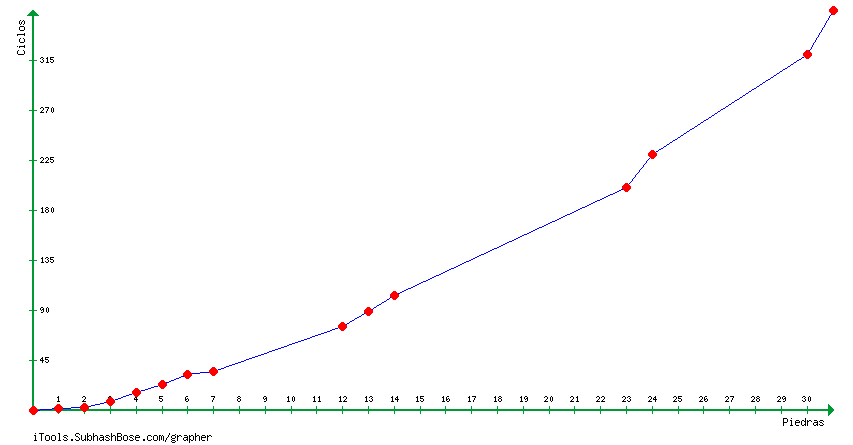
\includegraphics[width=15cm]{./graficos/grafico_ej3_0.png}
% grafico.eps: 0x0 pixel, 300dpi, 0.00x0.00 cm, bb=50 50 410 302
\end {center} 

Además, enfocandonos en el algoritmo de búsqueda DFS que realizamos luego de generar nuestro grafo, se puede observar como también la complejidad es lineal en relación a la cantidad de piedras:
\begin {center}
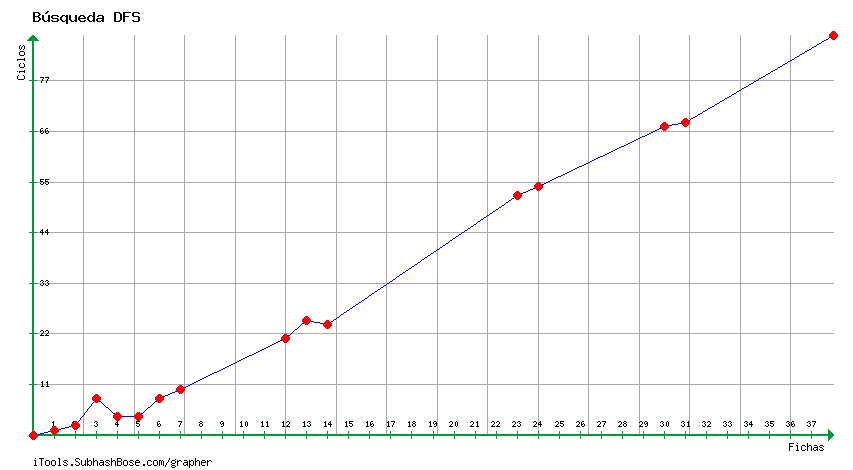
\includegraphics[width=15cm]{./graficos/grafico_ej3_1.png}
% grafico.eps: 0x0 pixel, 300dpi, 0.00x0.00 cm, bb=50 50 410 302
\end {center} 

Con lo cual, mediante un cantidad limitada de tests, se puede observar que el algoritmo propuesto para resolver el problema se comporta de la manera correcta y con la complejidad pedida.

\subsection{Conclusiones}
Como conclusión al problema dado en relación con la complejidad pedida, se pudo modelar un grafo a partir del simulacro de un sapo con el objetivo de llegar de desde una piedra de partida a otra de llegada, saltando entre distintas piedras a diferentes distancias con saltos limitados entre rangos; de tal forma que pueda encontrar un camino posible entre nodos, priorizando la performance temporal del algoritmo en vez de una solución más eficiente. En caso contrario, si se quiere buscar un camino mínimo, la complejidad aumentaría considerablemente. A pesar de ello, pudimos demostrar que además de que el algoritmo cumple lo pedido, para diferentes instancias con rangos, piedras y caminos variados, el algoritmo se suele comportar de la misma manera con complejidad lineal a la cantidad de piedras que tenga la instancia y esto es principalmente debido al algoritmo de búsqueda en profundidad usado que como máximo visitará todos los n nodos del grafo. 
